% Copyright (C)  2015  Alexander Jankowski, Philipp Hacker.
% Permission is granted to copy, distribute and/or modify this document
% under the terms of the GNU Free Documentation License, Version 1.3
% or any later version published by the Free Software Foundation;
% with no Invariant Sections, no Front-Cover Texts, and no Back-Cover Texts.
% The lincense itself can be found at <https://www.gnu.org/licenses/fdl-1.3>.

\documentclass[numbers=noenddot,a4paper,notitlepage,twoside,BCOR15mm]{scrartcl}
%\documentclass[numbers=noenddot,12pt,a4paper]{scrartcl}

\usepackage{ifoddpage}
\usepackage[infoshow]{tabularx}
\usepackage{fancyhdr}
\usepackage[greek,ngerman]{babel}
\usepackage[T1]{fontenc}
\usepackage[utf8]{inputenc}
\usepackage{libertine}
\usepackage{ziffer}
\usepackage{graphicx}
\usepackage{units}
\usepackage[infoshow]{tabularx}
\usepackage[all]{xy}
\usepackage{amsmath}
\usepackage{amssymb}
\usepackage{wrapfig}
\usepackage{upgreek}
\usepackage{esint}
\usepackage{float}
\usepackage[font=small,labelfont=bf]{caption}
\usepackage{subcaption}
\usepackage{lscape}
\usepackage{hyperref}
\usepackage{cleveref}
\usepackage{csquotes}
\usepackage[numbers]{natbib}

\renewcommand{\headrulewidth}{0.1pt}
\renewcommand{\footrulewidth}{0.1pt}
\newcommand{\name}{\text{Philipp Hacker}} %TODO Name des Protokollanten eintragen

\renewcaptionname{ngerman}{\figurename}{Abb. }
\renewcaptionname{ngerman}{\tablename}{Tab.}

\setlength{\parindent}{0pt}

\newcommand{\nummat}[1]{\left[\text{#1}\right]}
\newcommand{\num}[1]{$\left[\text{#1}\right]$}
\newcommand{\degree}{^\circ}
\newcommand{\diff}{\textnormal{d}}
\newcommand{\tenpo}[1]{ 10^{#1}}
\newcommand{\greek}[1]{\greektext#1\latintext}
\newcommand{\ix}[1]{_\text{#1}}
\newcommand{\imag}{\mathbf{i}}
\newcommand{\tilt}[1]{\textit{#1}}
\newcommand{\grad}[1]{\textit{grad}\left(#1\right)}
\newcommand{\divergenz}[1]{\textit{div}\left(#1\right)}
\newcommand{\euler}{\mathnormal{e}}
\newcommand{\fett}[1]{\textbf{#1}}
\newcommand{\einnup}{\hspace{0.2cm}}
\newcommand{\einnum}{\hspace{-0.2cm}}
\newcommand{\zentriert}[1]{\begin{center}#1\end{center}}
\newcommand{\ket}[1]{|#1\rangle}
\newcommand{\bra}[1]{\langle#1|}

\title{Protokoll: Mach-Zehnder Interferometer\\Quantenradierer} %TODO Name des Versuchs eintragen
\author{Alexander Jankowski, Philipp Hacker}
\date{\today}
\pagestyle{fancy}
\fancyhead[C]{\thepage}
\fancyhead[R]{\name}
\fancyfoot[C]{\thepage}
\fancyhead[L]{Abschnitt \thesection}


\begin{document}
	\maketitle
	\begin{center}
		Betreuer: Jakob Walowski\\ %TODO Name des Betreuers eintragen
		Versuchsdatum: 10.12.2015\\ %TODO Datum des Versuchs eintragen
		\begin{table}[h]
			\centering
			Note: %TODO Gute Note erhalten :)
			\begin{tabularx}{1.5cm}{|X|}
				\hline \\ \\
				\hline
			\end{tabularx}
		\end{table}
	\end{center}
	\vspace*{\fill}
	\tableofcontents
	\vfill
	\clearpage
	\section{Motivation}

		Ein sogenanntes \tilt{Mach-Zehnder}-Interferometer ist ein simpler, dennoch vielseitig einsetzbarer Aufbau zur Untersuchung von verschiedenen optischen Eigenschaften einer Probesubstanz. Des Weiteren kann ein MZI außerdem für die Visualisierung von Quantenmechanischen Phänomenen, wie bspw. dem Kollaps der Wellenfunktion und dem "`Welcher-Weg"'-Problem genutzt werden.\\
		Für diese Zwecke reicht es vollkommen aus, Bauteile mittlerer Güte mit einander geschickt zu kombinieren, um den gewünschten Effekt zu erhalten. Dabei verwendete man Strahlteiler, Polarisationsfilter, optische aktive Teile wie ein $\lambda/4$-Plättchen und einfache Spiegel.
	\clearpage
	\section{Physikalische Grundlagen}

		Das \tilt{Mach-Zehnder}-Interferometer dient hauptsächlich zur Untersuchung der Brechungsindizes von Probesubstanzen bspw. in flüssiger oder gasförmiger Phase. Dabei nutzt man das Prinzip der Interferometrie, bei welchem ein Lichtstrahl/eine elektromagnetische Welle über optische Bauteile zuerst in zwei Anteile gleicher Amplitude aufgeteilt und nach einer festen, bei beiden gleichen Wegstrecke wieder überlagert wird. Der eine Teil wird als Referenz zum anderen, durch eine Probe laufenden genutzt. Die gesuchten Informationen stecken hierbei in den relativen Phasen der Strahlen/Wellen.\\
		Bei dem Mach-Zehnder-Interferometer trifft ein kollimierter Lichtstrahl auf einen $50:50$-Strahlteiler, welcher einen Proben- und Referenzstrahl gleicher Intensitäten erzeugt. Idealer Weise legen diese, ohne das Einführen einer zu untersuchenden Substanz in den Strahlengang, einen gleichen optischen Weg im Aufbau zurück. Dabei werden sie zusätzlich über Spiegel jeweils einmal reflektiert und an einem zweiten Strahlteiler in 2 Detektoren gebracht. Den Aufbau dafür zeigt \autoref{img:aufbau}. Wichtig ist, dass die halb-verspiegelte Oberfläche des hinteren Teilers in Richtung des Detektors A/ersten Schirms, also von der Lichtquelle weg zeigt.

			\begin{figure}[H]
				\centering
				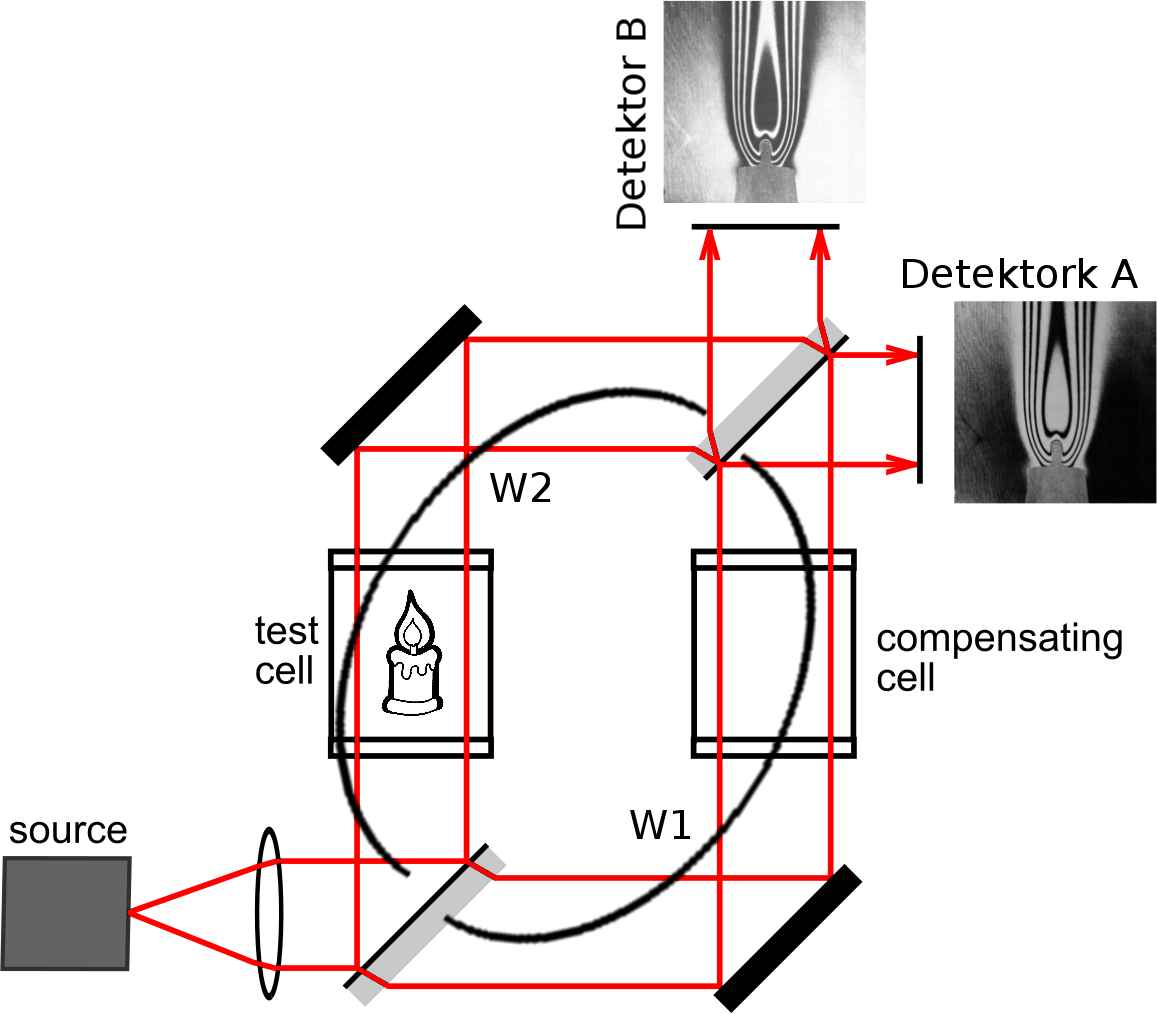
\includegraphics[width=0.7\textwidth]{Mach_Zehnder_interferometer.png}
				\caption{Schematischer Aufbau eines Mach-Zehnder-Interferometers. Ein kollimierter Lichtstrahl (\tilt{source}, Linse) trifft einerseits auf eine Probe (\tilt{test cell}) und andererseits auf eine leere Referenzkammer (\tilt{compensating cell}). Unterschiedliche Interferenzbilder werden auf 2 Schirmen, den Detektoren \fett{A} und \fett{B} nach Überlagerung beobachtet. \cite{WikiMZInt}}
				\label{img:aufbau}
			\end{figure}

\clearpage
			\subsection{MZ-Interferometer für Wellen}

				Nach \autoref{img:aufbau} durchläuft jeweils ein Strahl den Weg \fett{W1} und \fett{W2} mit den Weglängen $s\ix{W1}$ bzw. $s\ix{W2}$. Offensichtlich erfahren beide eine unterschiedliche Phasenverschiebung aufgrund der Probe bzw. den Reflexionen an Spiegeln und dem Durchgang durch die Strahlteiler.\\
				Bei der Reflexion eines Lichtstrahls einem optisch dichteren Medium - unter Annahme einer, zur Einfallsebene senkrecht polarisiert einlaufenden Welle und nicht-absorbierender Medien - tritt \enquote{für die zur Einfallsebene senkrechte Komponente ein Phasensprung von $\pi$ auf.} (aus \cite{MZdemt}, S. 239). Gleiches gilt auch für die Parallelkomponente und jeden Einfallswinkel (exc. den \tilt{Brewster-Winkel}) womit man annehmen kann: \enquote{Die Welle macht dann einen Phasensprung von $\pi$ bei der Reflexion.}\\
				Untersucht man nun die einzelnen Wege des Lichtstrahls - \fett{W1} oder \fett{W2} zum Detektor \fett{A} oder \fett{B} - so findet man, dass der gesamte Phasenunterschied jeweils $2\pi$ beträgt und man somit auf beiden Schirmen konstruktive Interferenz, e.g. \tilt{kohärente} Überlagerung  erwarten muss.\\
				Augenscheinlich muss zusätzlich die, bisher vernachlässigte Richtungsabhängigkeit eines Strahlteilers und der daran stattfindenden Reflexion beachtet werden. Es kommt demnach zu keinem Phasensprung bei einer Reflexion an der 'Rückseite', dem halb-durchlässigen Spiegel eines realen Strahlteilers. Andererseits: es findet keinen Phasensprung bei einer Reflexion an einem Medium, welches optisch Dünner ist.\\
				Tatsächlich nimmt eine durchlaufende Welle im Glas des Bauteils eine zusätzliche Phase von $2\pi s/\lambda$ auf, wobei $\lambda$ die Wellenzuglänge und $s$ der optische Weg im Medium - respektive Brechungsindex und Einfallswinkel - ist. Damit wird entlang des Pfades \fett{W1} zum Detektor \fett{A} die Gesamt-Phasenverschiebung zu $\varphi\ix{A}$ in \autoref{eq:phas1a}. Analog gilt dies für den anderen Detektor \fett{B} und den zweiten Pfad \fett{W2} in \autoref{eq:phas1b} - \autoref{eq:phas2b}.

					\begin{align}
						\varphi\ix{A}=&\pi+\pi+\frac{2\pi s}{\lambda}+\frac{2\pi s\ix{W1}}{\lambda} \label{eq:phas1a} \\
						\varphi\ix{B}=&\pi+\pi+\pi+\frac{2\pi s}{\lambda}+\frac{2\pi s\ix{W1}}{\lambda}=\phi\ix{1}+\pi \label{eq:phas1b} \\
						\vartheta\ix{A}=&\pi+\pi+\frac{2\pi s}{\lambda}+\frac{2\pi s\ix{W2}}{\lambda} \label{eq:phas2a} \\
						\vartheta\ix{B}=&\pi+2\frac{2\pi s}{\lambda}+\frac{2\pi s\ix{W2}}{\lambda} \label{eq:phas2b}
					\end{align}

			Mit der Kenntnis über die Phasen-\tilt{shifts} können nun eindeutig Interferenzverhältnisse vorhergesagt werden. Die Differenz aus $\varphi\ix{A}$ und $\vartheta\ix{A}$ entspricht gerade der Phasenrelation zwischen den Wellen entlang der beiden Pfade auf den Detektor \fett{A} in \autoref{eq:phasrel}. Gleiches gilt für die Überlagerung auf Schirm \fett{B} in \autoref{eq:phasrel2} \cite{MZwork}.

				\begin{align}
					\varphi\ix{A}-\vartheta\ix{A}=&\frac{2\pi (s\ix{W1}-s\ix{W2})}{\lambda}=\delta \label{eq:phasrel}\\
					\varphi\ix{B}-\vartheta\ix{B}=&\pi+\delta \label{eq:phasrel2}
				\end{align}

			Das Verhältnis ist nun sehr offensichtlich: für exakt gleiche optische Wegstrecken, dh. $\delta=0$ liegt auf \fett{A} konstruktive und an \fett{B} destruktive Interferenz vor! Jede Abweichung von diesem Idealfall verändert die Interferenzmuster auf beiden Schirmen. Des weiteren wandelt ein Unterschied in den Strahlteilern oder Spiegeln das Ergebnis nur dahingehend, als dass eine konstante Phase hinzu- oder abgezogen wird, was sich aber wiederum in $\delta$ verarbeiten lässt. Außerdem: liegen keine idealen 50:50-Strahlteiler vor, so gilt trotzdem die Regel des Phasensprungs, da damit die Energieerhaltung einher geht. Lediglich totale destruktive/konstruktive Interferenz wird damit verhindert \cite{MZwork}.\\
			Man kann die unterschiedlichen Interferenzerscheinung auf den Detektoren mit Hilfe der, bereits von \tilt{Albert A. Michelson} definierten Kontrastfunktion (\tilt{Sichtbarkeit}, 'visibility') in \autoref{eq:kontrastalt} mathematisch erfassen \cite{MZcohe}. Mit Hilfe der komplexen Selbst-Kohärenz-Funktion $\Gamma(\tau)$ für die Interferenz von 2 gleichsam intensive Wellen mit einer zeitlichen Beziehung $\tau$ - in Abhängigkeit ihrer Phasenverschiebung - einer monochromatischen Lichtquelle und dem dazugehörigen komplexen Grad der Selbst-Kohärenz $\gamma(\tau)$ ergibt sich\autoref{eq:kontrast}.

				\begin{align}
					&K=\frac{I\ix{max}-I\ix{min}}{I\ix{max}-I\ix{min}} \label{eq:kontrastalt} \\
					I\ix{max}(\tau)=2I\ix{1}+&2|\Gamma(\tau)| \,\, ;\quad I\ix{min}(\tau)=2I\ix{1}-2|\Gamma(\tau)| \nonumber \\
					K(\tau)=&\frac{|\left\langle E^*\ix{1}(t)E\ix{2}(t+\tau)\right\rangle|}{\left\langle E^*\ix{1}(t)E\ix{2}(t)\right\rangle}=\frac{|\Gamma(\tau)|}{\Gamma(0)}=|\gamma(\tau)| \label{eq:kontrast}
				\end{align}

			In der Regel \cite{MZcohe} ergeben bzw. beobachtet man, über die zeitliche Kohärenzbeziehung in $\tau$ monoton abfallenden Kontrastfunktionen. Dies ist insbesondere auch in dem Versuch dieses Experimentes der Fall.\\
			Ein weiterer Aspekt des Kontrast und der Interferenz ist die Polarisation, welche bspw. mit einem Polarisationsfilter eingestellt werden kann. Außerdem ist die Polarisation einer Lichtwelle beim Durchgang durch ein (optisch aktives) Medium nicht zwangsweise erhalten und kann auch bei der Reflexion (bspw. im \tilt{Brewster}-Winkel) sich ändern. 

			\subsection{MZ-Interferometer für einzelne Photonen}

				Nimmt man hingegen Abstand von der Welleninterpretation des Lichts, so wie es bisher angenommen wurde, und betrachtet das Experiment mit dem Mach-Zehnder-Interferometer auf quantenmechanische Weise, so ergibt sich sobald eine Frage der Art:

					\begin{quote}
						Wählt das Photon einen bestimmten Weg, wird es also vom Strahlteiler entweder durchgelassen oder reflektiert, und zeigt es so seine Teilcheneigenschaft, oder wird es sozusagen gleichzeitig durchgelassen und reflektiert, so dass es mit sich selbst interferiert und seine Wellennatur zeigt? \par\raggedleft ---\text{A. Schimony, Die Realität der Quantenwelt; 1996, S. 75 \cite{MZquote}}
					\end{quote}

				Betrachte man demnach nun ein einzelnes Photon im Zustand $\ket{\alpha}$ auf seinem Weg durch den Aufbau. Die jeweiligen Phasenverschiebungen kennen wir bereits aus \autoref{eq:phas1a} und folgende. Zu versehen sind die einzelnen Möglichkeiten zusätzlich noch mit, an die Normierung der Wahrscheinlichkeit geknüpften Faktoren $1/\sqrt{2}$, weswegen sich \autoref{eq:zust} und nachfolgende ergeben.

					\begin{align}
						\fett{W1, A:}&\quad \frac{1}{2}e^{\imag(2\pi+\phi+\theta\ix{W1})}\ket{\alpha}=\frac{1}{2}e^{\imag(\phi+\theta\ix{W1})}\ket{\alpha} \label{eq:zust} \\
						\fett{W1, B:}&\quad \frac{1}{2}e^{\imag(\phi+\theta\ix{W1}+\pi)}\ket{\alpha} \\
						\fett{W2, A:}&\quad \frac{1}{2}e^{\imag(\phi+\theta\ix{W2})}\ket{\alpha} \\
						\fett{W2, B:}&\quad \frac{1}{2}e^{\imag(\pi+2\phi+\theta\ix{W2})}\ket{\alpha}
					\end{align}

				Unter der Annahme, dass die optischen Wege gleich sind, e.g. $\theta\ix{W2}=\theta\ix{W1},$ können deren Phaseneinflüsse vernachlässigt werden - man könnte genau so gut den Zustand $\ket{\beta}=e^{\imag\theta}\ket{\alpha}$ definieren.\\
				Die Wahrscheinlichkeit, dass ein Photon also auf den Detektor \fett{A} bzw. \fett{B} trifft, ist demnach die Summe der beiden Möglichkeiten, auf \fett{W1} bzw. \fett{W2} zu propagieren. Es hat also eine nicht-verschwindende Probabilität, beide Wege gleichzeitig zu begehen, um dann an den Detektoren "`mit sich selbst zu interferieren"'. Natürlich ist hierbei von keinem "`Weg des Photons"' oder Selbstinterferenz zu sprechen, da die Beobachtung auf dem Schirm bzw. eine Messung auf einem Pfad den Kollaps der Wellenfunktion zur Folge hat und den Wellen- bzw. Teilchencharakter damit zerstört (je nach Betrachtungsweise).\\
				Mit Hilfe eines Polarisators auf dem Weg \fett{W1} nach der Strahlteilung kann man zudem das \enquote{Welchen-Weg-Problem} nachvollziehen: aus dem anfänglichen Zustand $\ket{\alpha}$ wird somit ein \tilt{Hilbert}-Vektor $\ket{\gamma}$, verziert mit der gleichen Phasenverschiebung wie zuvor (\autoref{eq:zust}). Die Gesamt-Wahrscheinlichkeit ist in \autoref{eq:wahr} gegeben, wobei die Bedingung $|\frac{1}{\sqrt{2}}e^{\imag\phi}|^2=1/2$ an den Phasenhub geknüpft werden muss. Diese ist somit gleichbedeutend mit der Wahrscheinlichkeit, ein Photon auf dem Detektor \fett{A} zu messen. Durch die Kenntnis, bzw. das Aufprägen der Polarisation des Photons 'kann' damit prinzipiell eine Weginformation im Interferometer erhalten werden.

					\begin{align}
						\frac{1}{2}e^{\imag\phi}\ket{\gamma}+\frac{1}{2}e^{\imag\phi\ket{\alpha}}=\frac{1}{\sqrt{2}}e^{\imag\phi}\left(\frac{1}{\sqrt{2}}\ket{\gamma}+\frac{1}{\sqrt{2}}\ket{\alpha}\right) \label{eq:wahr}
					\end{align}

				In diesem Experiment werden hingegen 2 Polarisatoren auf \fett{W1} und \fett{W2} benutzt, um gezielt die Interferenz eines Photons mit sich selbst zu verhindern. Durch die vollständige Einschränkung des Polarisationszustandes kommt es, wie zuvor angedeutet, zum Kollaps der Wellenfunktion. Das System der Wellenfunktionen (Hilbert-Vektoren) geht in einen diskreten Zustand eines Teilchens über.\\
				Ein weiterer Polarisator kann genutzt werden, um die Information über den Verlauf des Photons "`auszuradieren"' (\tilt{quantum eraser}, Quantenradierer). Dieser wird dafür hinter dem zweiten Strahlteiler vor einem Detektor platziert. Damit ist es wieder möglich, Interferenzmuster zu beobachten.

	\clearpage
	\section{Durchführung}

		Der Versuch zum \tilt{Mach-Zehnder-Interferometer} ist aus 3 Teilen aufgebaut.\\
		Zum Beginn des Experimentes gilt es sich mit dem optischen Aufbau nach \cite{MZaufbau} vertraut zu machen und die verwendeten, optischen Bauteile zu charakterisieren. Dafür wird der Polarisationsgrad des eingebauten Helium-Neon-Lasers ($\unit[0,2\dots1]{mW}$) und die Polarisation nach dem Durchgang durch einen Polarisator bei maximaler Intensität bestimmt. Dafür kann eine arbiträre Photodiode und Multimeter benutzt werden. Im Anschluss daran muss das sog. $\lambda/4$-Plättchen untersucht werden: mit Hilfe der Polarisatoren wird jenes so eingestellt, das zirkular polarisiertes Licht vorliegt.\\
		Im zweiten Teil gilt es, den Aufbau nach \cite{MZaufbau} vorzunehmen. Hierbei ist die möglichst horizontale und, innerhalb des Aufbaus parallele Strahlführung von großer Bedeutung. Sowohl Winkel und Höhe der Strahlteiler, Spiegel als auch der Linse (notwendig um \tilt{Fresnelringe} auf dem Schirm zu beobachten) sind hierbei zu beachten.\\
		Wurde eine optimale Interferenz der Teilstrahlen am zweiten Strahlteiler/auf beiden Schirmen erreicht, so kann mit einer CCD-Kamera das beobachtete Muster aufgenommen werden. Daraus lässt sich ebenfalls die Kontrastfunktion ablesen.\\
		Schließlich kann mit den, in \autoref{img:aufbau2} mit \fett{PF1} bis \fett{PF3} bezeichneten Polarisatoren der \tilt{Quantum Eraser} aufgebaut werden.

			\begin{figure}[H]
				\centering
				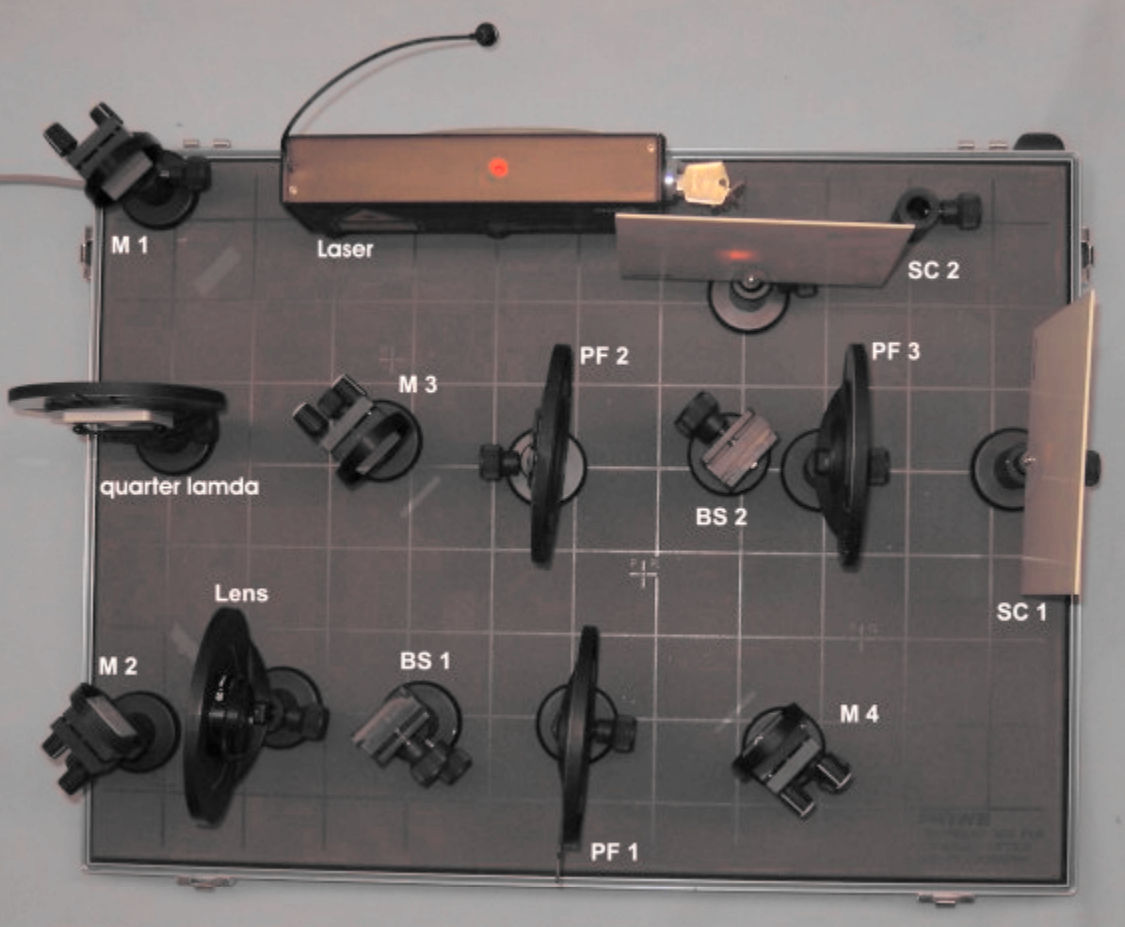
\includegraphics[width=0.85\textwidth]{aufbau.png}
				\caption{Aufbau des finalen Experimentes nach \cite{MZaufbau}. Das $\lambda/4$-Plättchen entspricht dem \tilt{quarter lambda}, die Spiegel den \fett{M1} bis \fett{M4} und die Strahlteiler den \fett{BS1} und \fett{2}. Beobachtet wird die Intereferenz auf \fett{SC1} und \fett{SC2}.}
				\label{img:aufbau2}
			\end{figure}

	\clearpage
	\section{Auswertung}
	
	\subsection{Polarisationsgrad des Laserlichtes}
	
	Zur Bestimmung der Polarisation wird die Intensität des durch einen Polarisator transmitierten Laserlichtes gemessen. Die aufgenommenen Werte sind in \autoref{fig:1xpol} dargestellt. Die Intensität weist bei kleinen Winkeleinstellungen auf. Weiterhin ist zu beobachten, dass die Intensität in beide Richtungen gleichermaßen abnimmt, bis sie jeweils bei einem Winkel von ca. $90^\circ$ in ein Minimum läuft. Um den Polarisationgrad zu bestimmen kann die Beziehung
	\begin{equation}
		K = \frac{I_\mathrm{max}-I_\mathrm{min}}{I_\mathrm{max}+I_\mathrm{min}}
		\label{eq:kontrast}
	\end{equation}
	verwendet werden, welche den Kontrast $K$ in Abhängigkeit der minimalen und maximalen Intensität $I_\mathrm{max}$, $I_\mathrm{min}$ setzt. Je höher der gemessene Kontrast ist, desto näher ist das Licht total Polarisiert. Für diese Messung wird als minimale Intensität ein Wert von $I_\mathrm{min} = 0,2$ und als maximale Intensität $I_\mathrm{max} = 33,0$ aufgenommen. Der zugehörige Kontrast ist $K \approx 0,99$, weshalb man von quasi vollständig polarisierten Laserlicht ausgehen kann.
	
	\begin{figure}[h]
		\centering
		\begin{subfigure}{.49\textwidth}
			\centering
			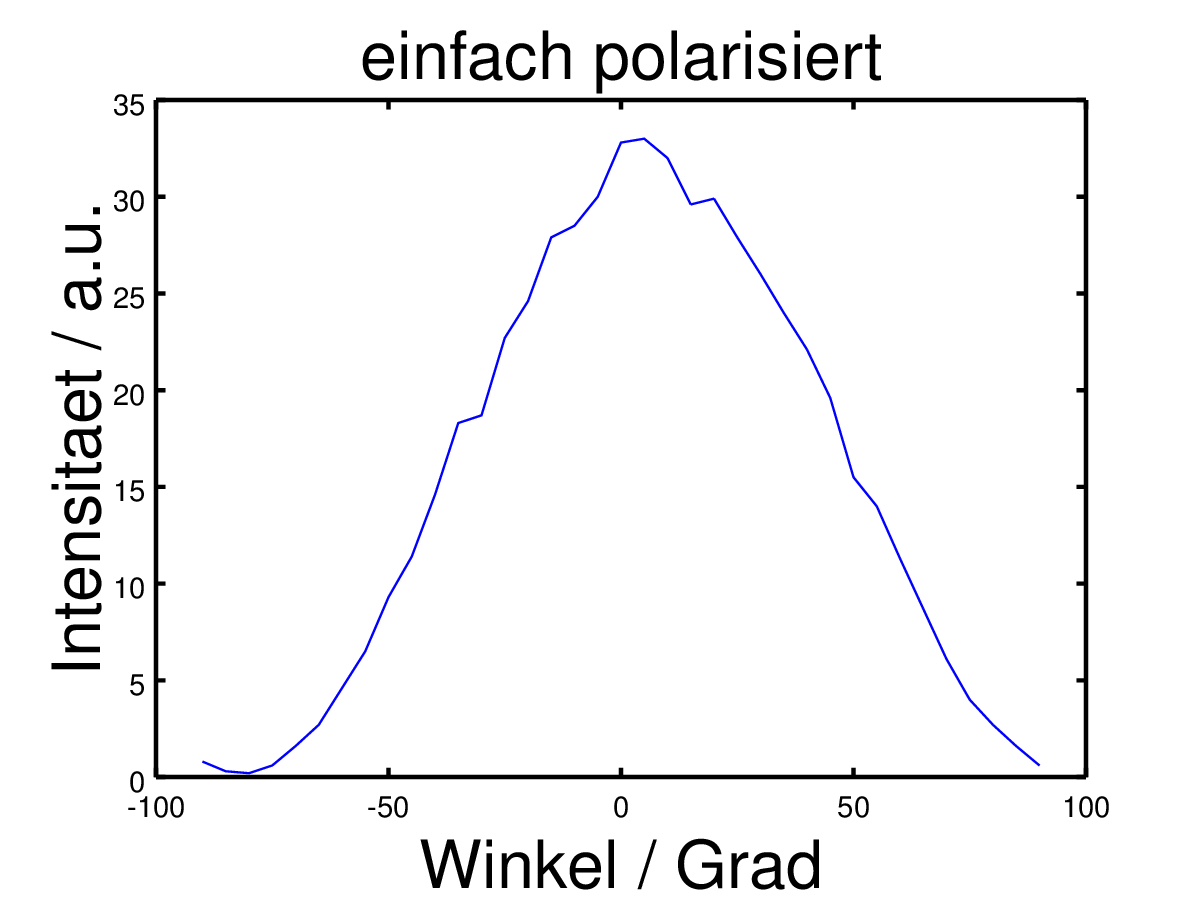
\includegraphics[width=0.8\linewidth]{pics/1xpol.png}
		\end{subfigure}
		\begin{subfigure}{.49\textwidth}
			\centering
			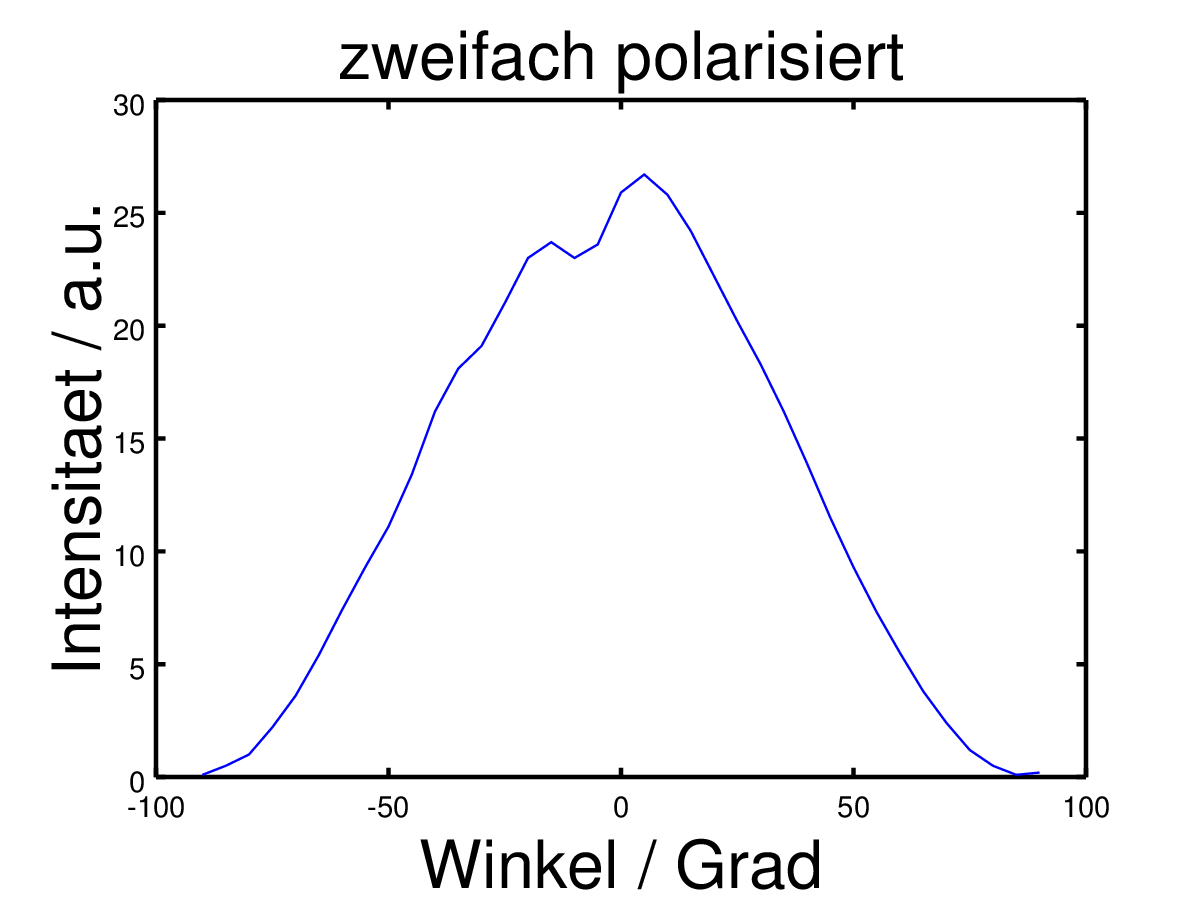
\includegraphics[width=0.8\linewidth]{pics/2xpol.png}
		\end{subfigure}
		\caption{Intensität des Laserlichtes nach dem Durchgang eines bzw. zwei Polarisatoren in Abhängigkeit der Einstellungsinkel.}
		\label{fig:1xpol}
	\end{figure}
	
	Weiterhin sind ist der Intensitätsverlauf des Lichtes nach Durchgang durch das $\lambda/4$-Plättchen und eines auf $0^\circ$ eingestellten Polarisators in Abhängigkeit des Einstellungswinkels des Plättchens in \autoref{fig:lambda4} dargestellt. Die Messung zeigt, das dass $\lambda /4$-Plättchen, nicht wie erwartet bei $45^\circ$ zirkular polarisiertes Licht erzeugt, sondern bei einem Winkel von ca. $50^\circ$. Für die weiteren Messung wird diese Einstellung verwendet. \clearpage
	
	\begin{figure}[h]
		\centering
		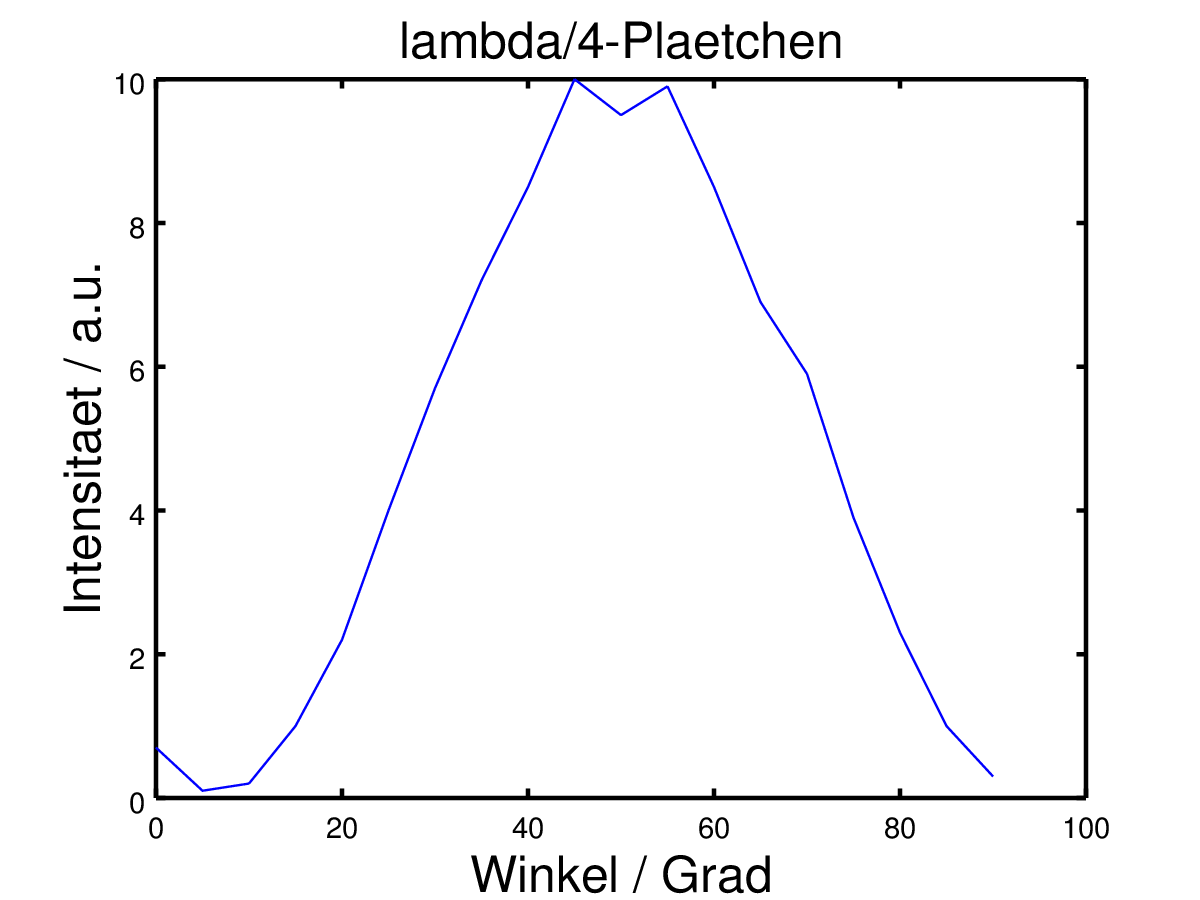
\includegraphics[width=0.5\columnwidth]{pics/lambda4.png}
		\caption{Intensität des Laserlichtes nach dem Durchgang durch das $\lambda /4$-Plättchen und einen auf $0^\circ$ eingestellten Polarisator. Bei der Messung wurde der Einstellungswinkel des $\lambda /4$-Plättchens variiert.}
		\label{fig:lambda4}
	\end{figure}
	
	\subsection{Kontrastfunktion des Mach-Zehnder-Interferometers}	
	
	Nach dem Aufbau des Mach-Zehnder-Interferometers wird das Interferenzmuster mit einer Kamera aufgenommen. Dieses ist ohne einsetzen der Polarisatoren in \autoref{fig:ohnealles} dargestellt. Es war im Zeitrahmen des Versuches nicht möglich ein Interfenzmuster mit Ringen zu erzeugen und es wurde sich mit den dargestellten Muster zufrieden gegeben. 
	
	\begin{figure}[h]
		\centering
		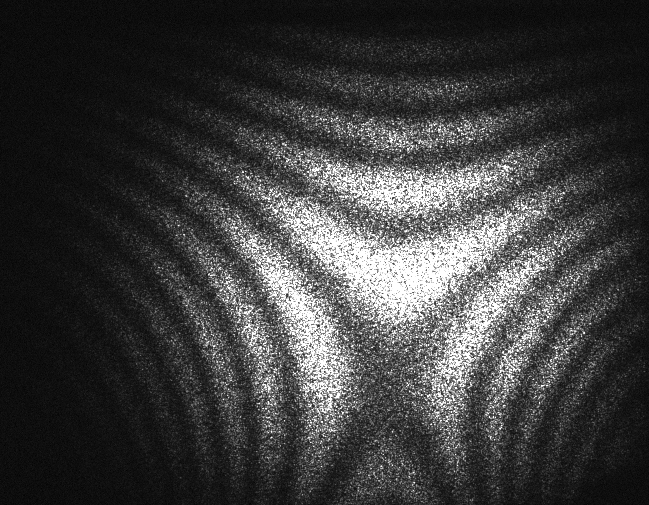
\includegraphics[width = 0.5 \columnwidth]{pics/ohnealles.png}
		\caption{Interferenzmuster des rekombinierten Laserlichtes an einem der Schirme aufgenommen mit einer CCD Kamera in Graustuffen.}
		\label{fig:ohnealles}
	\end{figure}
	
	Nach dem Einbau der Polarisatoren werden Aufnahmen bei verschiedenen Einstellungswinkel vorgenommen, wobei der Winkel von $0^\circ$ bis $90^\circ$ in $5^\circ$ Schritten variiert wird. In \autoref{fig:interpol} sind die Interferenzmuster vom minimalen und maximalen Winkel zur Veranschaulichung gegenüber gestellt. Ein Querschnitt durch diese Bilder ist in \autoref{fig:test} für ausgewählte Winkel dargestellt. Der Querschnitt wurde hierbei für jeden Fall an der gleichen Stelle angefertigt. Es ist bereits mit dem Auge zu erkennen, das der Kontrast bei größeren Winkeln abnimmt und für die Messung bei $90^\circ$ ist bereits kein Interferenzmuster mehr zu erkennen. An Hand der Querschnitte kann mit Hilfe von \autoref{eq:kontrast} der Kontrastverlauf der Messung aufgetragen werden. Das Ergebnis ist in \autoref{fig:kontrast} dargestellt.
	
	\begin{figure}
		\centering
		\begin{subfigure}{.49\textwidth}
			\centering
			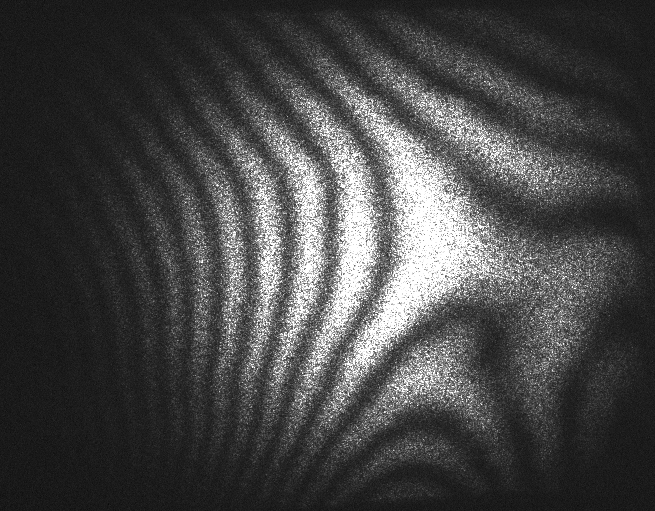
\includegraphics[width=.7\linewidth]{pics/0grad_.png}
		\end{subfigure}
		\begin{subfigure}{.45\textwidth}
			\centering
			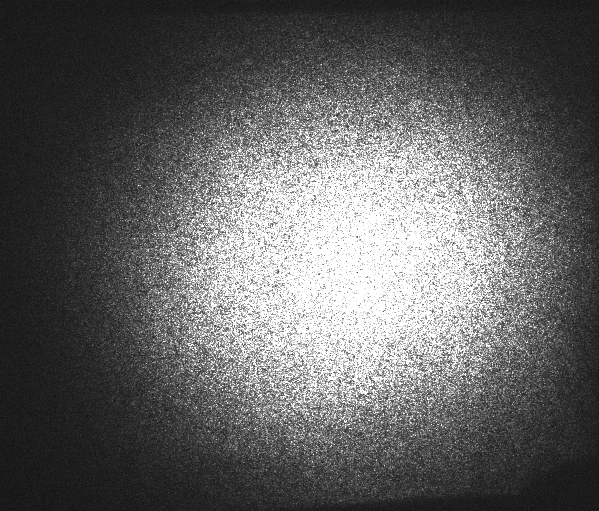
\includegraphics[width=.7\linewidth]{pics/90grad_.png}
		\end{subfigure}	
		\caption{Interfentmuster des rekombinierten Laserlichtes nach dem Einsetzten der Polarisatoren bei einer Winkeleinstellung von $0^\circ$ bzw. $90^\circ$ in Graustuffen.}
		\label{fig:interpol}
	\end{figure}
	
	
	\begin{figure}
		\centering
		\begin{subfigure}{.49\textwidth}
			\centering
			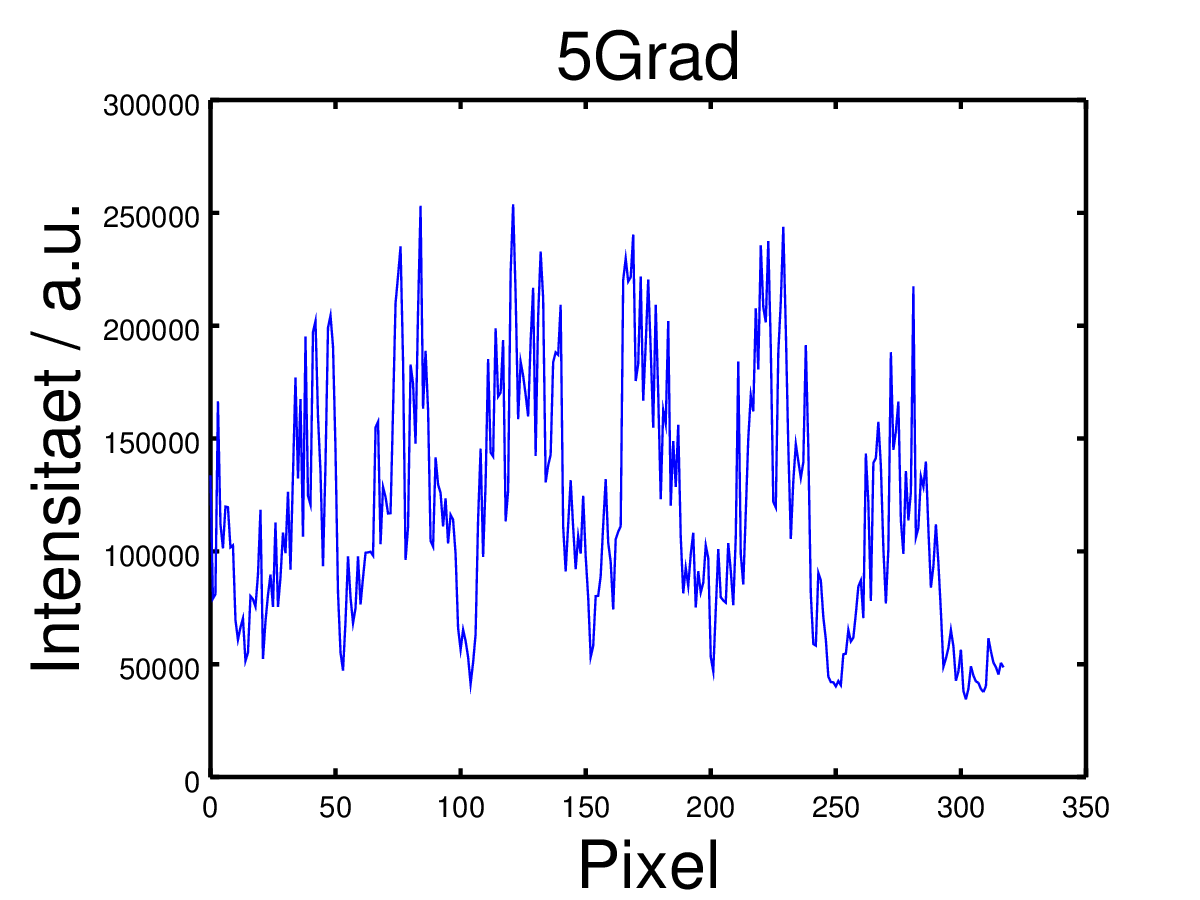
\includegraphics[width=0.75\linewidth]{pics/5grad.png}
		\end{subfigure}
		\begin{subfigure}{.49\textwidth}
			\centering
			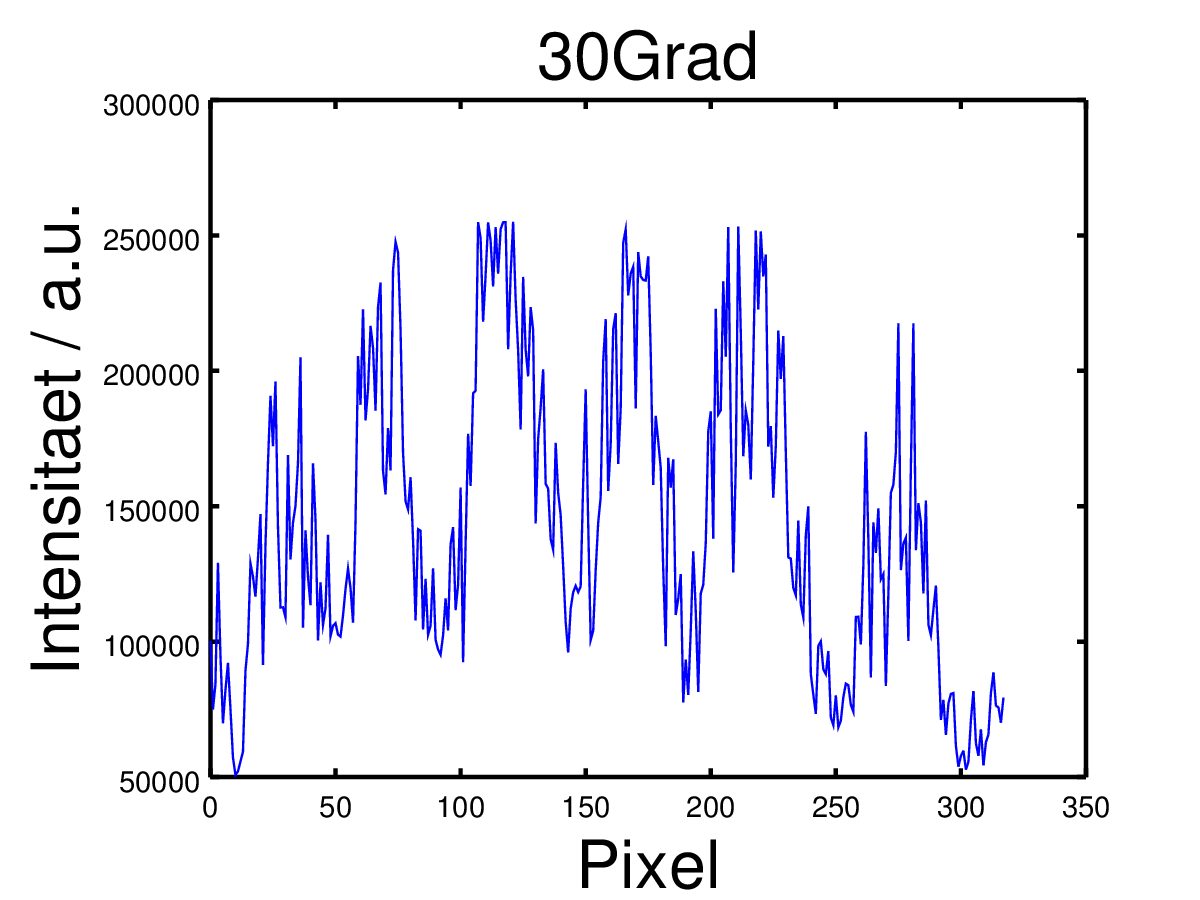
\includegraphics[width=0.75\linewidth]{pics/30grad.png}
		\end{subfigure}
		\begin{subfigure}{.49\textwidth}
			\centering
			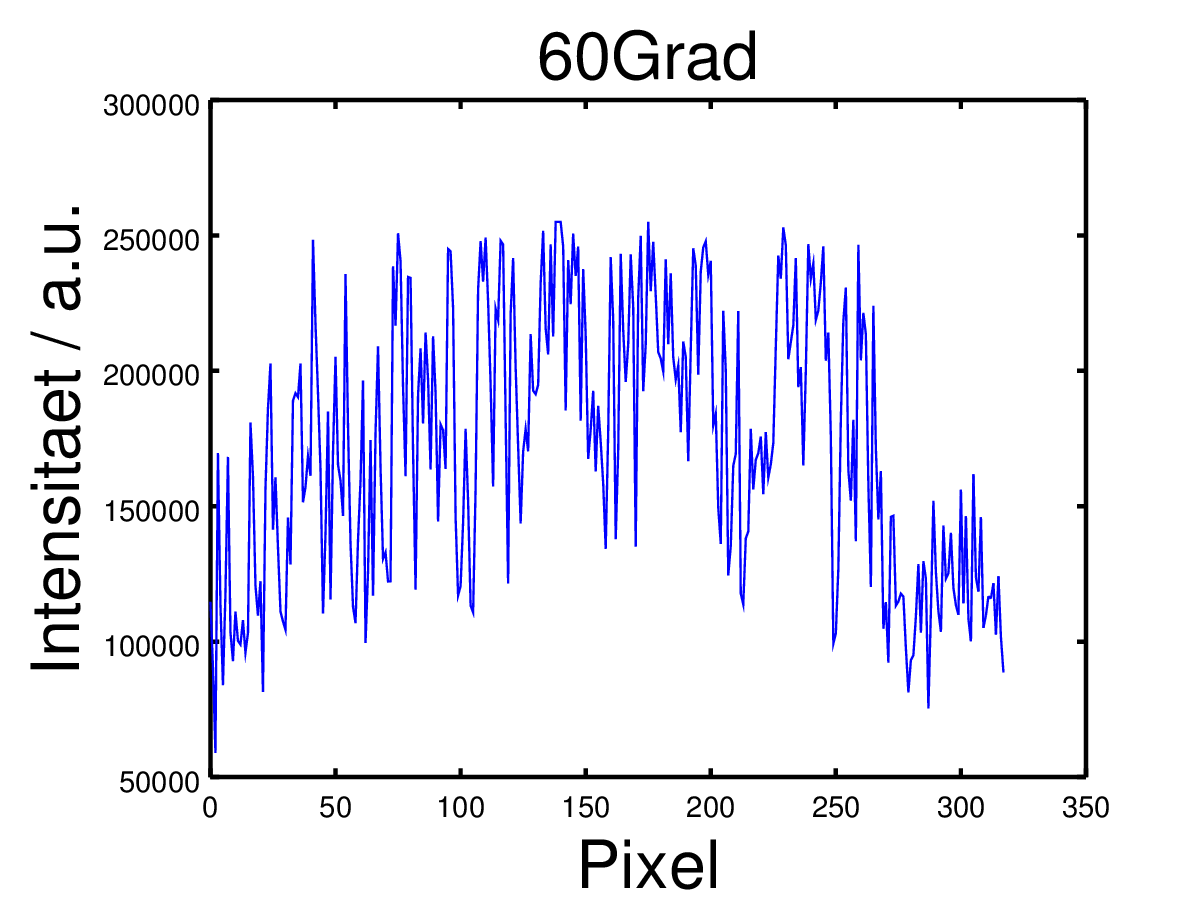
\includegraphics[width=0.75\linewidth]{pics/60grad.png}
		\end{subfigure}
		\begin{subfigure}{.49\textwidth}
			\centering
			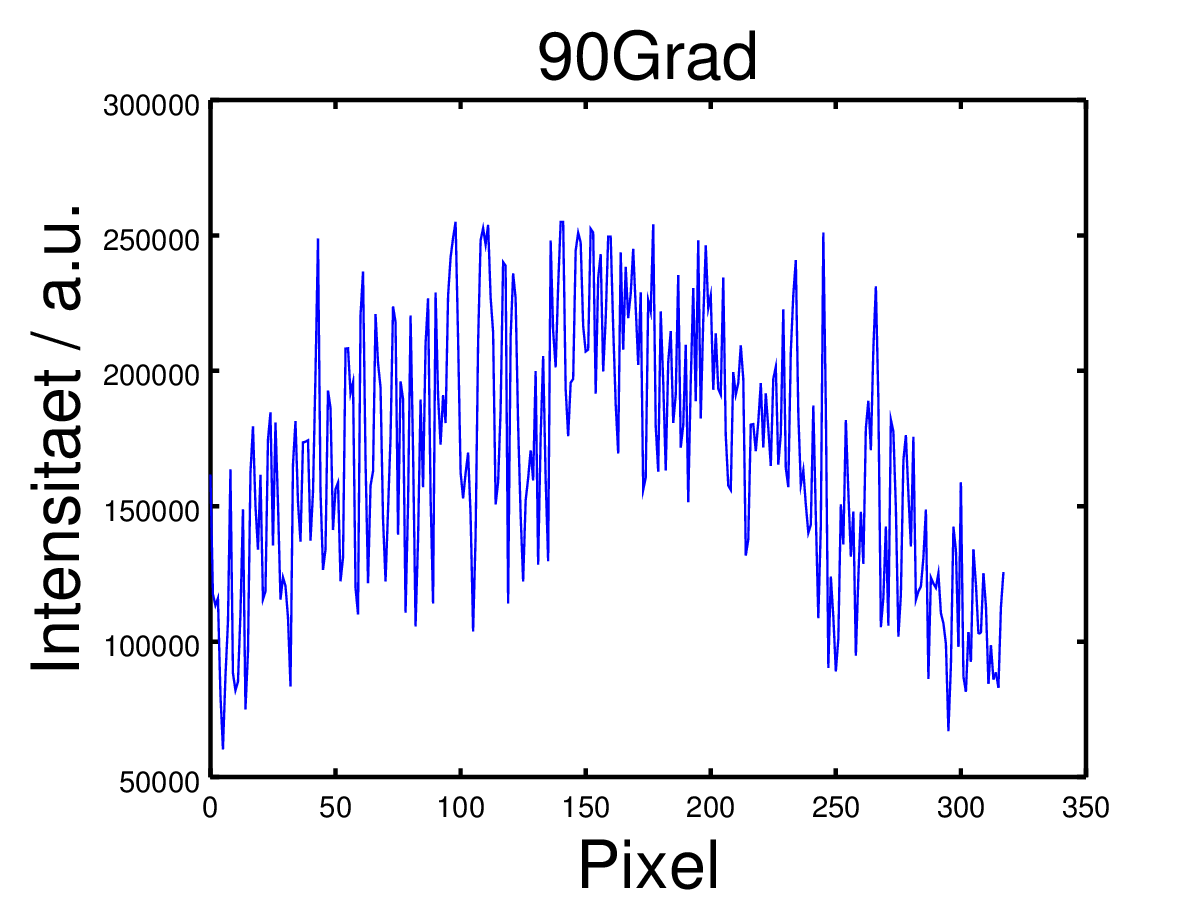
\includegraphics[width=0.75\linewidth]{pics/90grad.png}
		\end{subfigure}
		\caption{Intensitätsprofil des Interferenzmusters entlang einer Graden für verschiedene Winkeleinstellung des Polarisators.}
		\label{fig:test}
	\end{figure}
	
	\begin{figure}
		\centering
		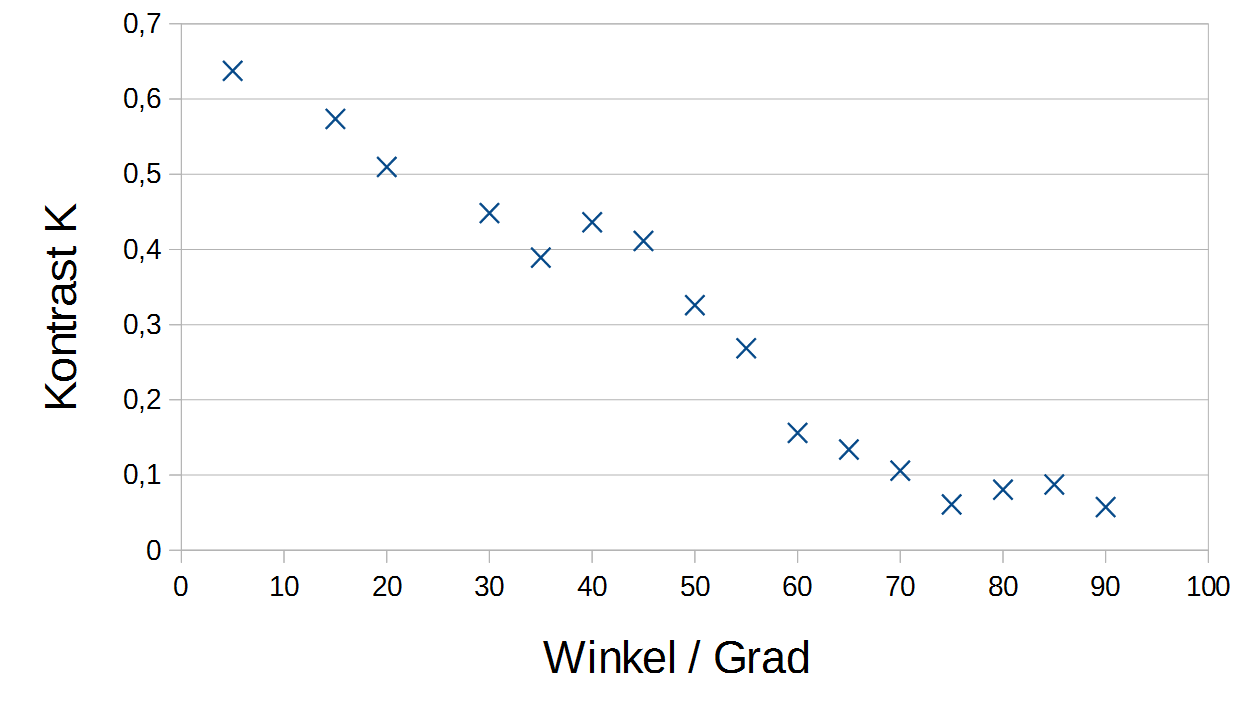
\includegraphics[width=0.8\columnwidth]{pics/Kontrast.png}
		\caption{Kontrast des Interfenzmusters in Abhängigkeit des Einstellungswinkels des Polarisators.}
		\label{fig:kontrast}
	\end{figure}
	\newpage
	\subsection{Diskusion der Ergebnisse}
	
	Der Kontrastverlauf in \autoref{fig:kontrast} fällt zwar mit zunehmenden Winkel ab, schwankt aber stark. Der Hauptgrund für diese Schwankungen ist eine schlechte Belichtung der Aufnahme. Die intensivsten Maxima in den Bildaufnahmen sind stark überbelichtet und übersteigen das Maximum der Intensität, welche einen arbiträren Zahlenwert von $255$ hat. Dadurch kann der Kontrast nicht im Zentrum des Bildes gemessen werden, sondern wird möglichst nahe am diesem angesetzt. Diese Intensitätsprofile haben jedoch starke Schwankungen, wodurch der Kontrast für die einzelnen Winkeleinstellungen nur approximativ bestimmt werden kann.\\
	Weiterhin konnte im Zeitrahmen des Versuches der Aufbau des Quantenradierers nicht mehr realisiert werden, wodurch eine Auswertung einer solchen Messung ausbleibt.
	
	\newpage
	\section{Anhang}
	
	\bibliography{all.bib}
	\bibliographystyle{unsrt}
	
\end{document}